\section{Zielsetzung}
  \label{sec:Zielsetzung}
  Im Versuch wird aus experimentellen Daten die Temperaturabh"angigkeit der Relaxationszeit $\tau(T$) der Dipole im einwertigen Ionenkristall KBr(Sr) (dotiert mit zweiwertigen Strontium-Ionen) bestimmt.
  Daf"ur wird der Dipolarisationsstrom des Kristalls $i(T)$ in Abh"angigkeit von der Temperatur $T$ des Kristalls gemessen.

  Durch Anpassen von zwei Verläufen an die Messwerte wird die Aktivierungsenergie $W$ der Dipole auf zwei Arten bestimmt.
  %An die erhaltenen ($i(T),T$)-Wertepaare werden zwei Theorieverl"aufe gefittet und so durch Augleichsrechnung die Aktivierungsenergie der Dipole $W$ auf zwei verschiedene Arten bestimmt.
  Aus den Messdaten wird auch die charakteristische Relaxationszeit $\tau_0$ bestimmt, mit $\tau_0$ und $W$ ist $\tau(T)$ bekannt.





\section{Theorie}
  \label{sec:Theorie}

  \subsection{(Entstehung der) el. Dipole in Ionenkristallen}
    Bei der Dotierung von einem Ionenenkristall aus einwertigen Ionen mit zweiwertige Ionen (z.B. $\text{Sr}^{2+}$) entstehen permanente elektrische Dipole (Abb. \ref{fig;dipole}).
    Mit jedem zweiwertigen Kation/Anion im Kristall ensteht auch eine Leerstelle/Abwesenheit eines Atoms an der Position eines einweritgen Kations/Anions des Kristalls, um die Ladungsneutralit"at zu erhalten.
    Die Dotierungsionen bilden mit den neutralen Leerstellen elektrische Dipole $\vec{p}$, welche durch
    \begin{equation}
      \vec{p}=ql\vec{n_p}=p\vec{n_p}
      \label{dipol}
    \end{equation}
    beschrieben werden k"onnen.
    Hierbei ist $q$ die Ladungsdifferenz , $l$ der Abstand der Punktladungen und $\vec{n_p}$ Richtungsvektor, gegeben durch die Verbindungsachse zwischen Ion und Leerstelle (Abb. \ref{fig:dipole}).
    \begin{figure}[H]
      \centering
      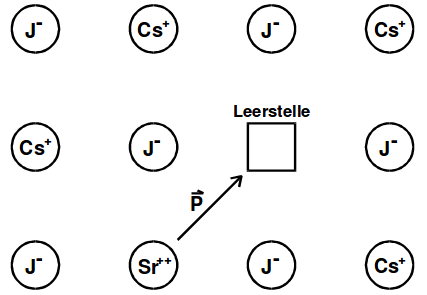
\includegraphics[height=5cm]{bilder/Dipole.png}
      \caption{Entstehung und Diskretisierung der Raumrichtungen von elektrischen Dipolen in dotierten Ionenkristallen (dotiert mit $\text{Sr}^{2+}$) \cite{Anleitung}.}
      \label{fig:dipole}
    \end{figure}
    Wegen festen Gitterpl"atzen k"onnen die Dipole nur in diskrete Richtungen orientiert sein, welche allerdings statistisch verteilt sind, sodass die Polarisation $P$, also das Gesamtdipolmoment pro Volumen,
    \begin{equation}
      \vec{P}=\frac{\sum\nolimits_{n=0}^N \vec{p_n}}{V}
      \label{polarisation}
    \end{equation}
    verschwindet.

    Experimentell wurde festgestellt, dass die Dipole bei Temperaturen unter $\SI{500}{K}$ praktisch nur durch die Bewegung der Leerstellen im Kristall ihre Richtung "andern k"onnen.
    Dabei muss der Dipol aber, wegen des periodischen Verlaufes des Gitterpotentials, mindestens eine bestimmte (materialspeziefische) Energie, die sogenannte Aktivierungsenergie $W$, haben.
    Der Anteil aller Dipole, welcher bei der Temperatur $T$ des Materials mindestens diese Energie hat, ist gegeben durch die Boltzmann-Verteilung:
    \begin{equation}
      \text{e}^{\frac{W}{k_BT}}
      \label{relaxationszeit}
    \end{equation}
    Die Boltzmanverteilung gibt die Energieverteilung der Gasteilchen im klassischen idealen Gas bei der Temperatur $T$ an bzw. die Wahrscheinlichkeit, dass ein Teilchen im idealen Gas mit Temperatur $T$ die Energie $W$ hat.




  \subsection{Die Relaxationszeit der Dipole eines Materials}
    Als Relaxationszeit wird die mittlere Zeit zwischen zwei Umorientierungen eines Dipols im Kristall bezeichnet.
    Wegen der Boltzmann-Verteilung, ist sie eine Funktion der Temperatur $T$ folgender Form:
    \begin{equation}
      \tau(T) = \tau_0 \text{e}^{\frac{W}{k_BT}}
      \label{relaxzeit}
    \end{equation}
    mit der charakteristischen Relaxationszeit $\tau_0$.\\
    \\Zur (experimentellen) Bestimmung von $\tau_0$ und $W$ ist die Aufnahme des Depolarisationsstroms $i(T)$ als Funktion der Temperatur $T$ notwendig.
    Dieser wird beobachtet, wenn sich die Dipole im Kristall, nach vorheriger Ausrichtung entlang eines angelegten elektrischen Feldes (Polarisation), im Laufe der Zeit wieder in statistisch orientierte Richtungen ausrichten, sodass die Polarisation $P$ wieder auf null sinkt.
    Dieser Vorgang wird als Dipolrelaxation bezeichnet.

    Der Depolarisationsstrom $i(T)$ wird zun"achst steil mit der Temperatur anwachsen, da die Relaxationszeit exponentiell mit der Temperatur abnimmt, wie in Gleichung (\ref{relaxzeit}) zu sehen.
    Dann wird er abfallen, weil immer weniger Dipole noch nicht relaxiert sind.
    Der Depolarisationsstrom $i(T)$ wird bei Messbeginn und zum Ende der Messung nicht den Wert null annehmen, denn f"ur endliche Temperaturen ($T>0 \implies \tau(T) \neq \infty$) findet immer eine Umorientierung der Dipole z"uruck in die statistische Richtungsverteilung statt, was f"ur einen Untergrundstrom sorgt.
    %Dabei beginnt und endet der Depolarisationsstrom $i(T)$ aber nicht genau bei null, wegen Untegrund, z.B. weil auch f"ur tiefe Temperaturen ($T>0$) ein Depolarisationstrom flie"st ($\tau(T) \neq \infty$).
    Dieser Untergrund muss in der Praxis durch Subtrahieren einer geeigneten Funktion von den Messwerten eleminiert werden.
    Weiterhin kann der Graph in der Praxis auch zwei lokale Maxima haben, durch einen zweiten Relaxationsprozess mit einer h"oheren Aktivierungsenergie $W$, der also bei h"oheren Temperaturen beginnt.
    Dann wird die Temperatur, bei der das lokale Minimum von $i(T)$ zwischen den beiden lokalen Maximan vorliegt, $T^*$ gennant.
    %Die Temperatur des Minimums ist $T^*$.
    Ein einfacher Verlauf mit nur einem Aktivierungsprozess ist qualitativ in Abb. \ref{fig:depolstrom} dargestellt.
    \begin{figure}[H]
      \centering
      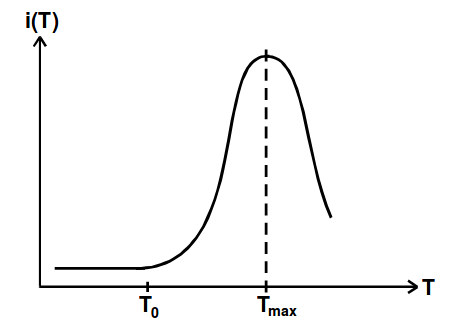
\includegraphics[height=5cm]{bilder/Depolarisationsstrom.png}
      \caption{Der Depolarisationsstrom in Abh"angigkeit der Temperatur \cite{Anleitung}.}
      \label{fig:depolstrom}
    \end{figure}



    \subsubsection{Ermittlung der Aktivierungsenergie $W$ aus der Depolarisationsstromdichte $j(T)$ (Methode 1)}
      Die Depolarisationsstromdichte $j(T)$ ist gegeben durch
      \begin{equation}
        j(T) = \frac{i(T)}{F} = y(T_p)\cdot p \cdot\frac{\text{d}N}{\text{d}t} \; .
      \end{equation}
      Hierbei ist $F$ die Querschnittsfl"ache der Kristallprobe, $p$ ist der Betrag eines Dipolmomentes (\ref{dipol}) im Kristall, also eine Materialeigenschaft,
      $\text{d}N/\text{d}t$ ist die Zahl der im Mittel pro Zeit bei der Temperatur $T$ relaxierenden Dipole.
      $y(T,E)$ ist der Bruchteil aller Dipole die bei angelegtem elektrischen Feld $E$ in Feldrichtung ausgerichtet sind. Dieser Anteil entspricht nicht 100\%, weil die Ausrichtung der Dipole durch die thermische Bewegung der Gitteratome gest"ort wird.
      F"ur den Fall, dass $pE<<k_BT$ (hier gegeben) ist $y$
      \begin{equation}
        y(T_p,E) \approx \frac{pE}{3k_BT_p}
      \end{equation}


      Nach Umformungen und einer weiteren N"aherung ergibt sich $j(T)$ zu:
      \begin{equation}
          \text{ln}(j) = \text{ln}\left( \frac{p^2E}{3k_BT_p}\frac{N_p}{\tau_0} \right) + \frac{-W}{k_B}\frac{1}{T}
        \label{depolarisationsstromdichte}
      \end{equation}
      Wird ln(j(T)) gegen $1/T$ aufgetragen (Logarithmierung beider Seiten), kann man in dem Bereich, wo diese N"aherung g"ultig ist eine Gerade beobachten.
      Durch Anpassen von
      \begin{align}
        y &= c + mx\\
        &\text{mit}\\
        m &=-\frac{W}{k_BT}, \: b=\text{ln}\left( \frac{p^2E}{3k_BT_p}\frac{N_p}{\tau_0} \right)
        \label{methode1}
      \end{align}
      an diesen Bereich, kann $W$ daher aus der Steigung der Ausgleichsgeraden berechnet werden.


    \subsubsection{Ermittlung Aktivierungsenergie $W$ aus der Polarisation $P$ der Probe (Methode 2)}
      Um $W$ mit gr"o"serer Genauigkeit aus dem gesamten Kurvenverlauf $i(T)$ zu ermitteln, kann man die Polarisation $P$ der Kristallprobe betrachten.
      Da die Polarisation proportional zur Zahl der orientierten Dipole ist, wie es in Gleichung (\ref{polarisation}) zu sehen ist, gehorcht sie der Relaxationsgleichung
      \begin{equation}
        \frac{\text{d}P}{\text{d}t} = \frac{P(t)}{\tau(T(t))} \;.
        \label{polarisation_relaxation}
      \end{equation}
      F"ur den Polarisationsstrom $i(T(t))$ gilt:
      \begin{equation}
        i(t) = F\frac{\text{d}P}{\text{d}t} \: ,
        \label{polarisationsstrom(t)}
      \end{equation}
      mit dem Probenquerschnitt $F$.
      Durch Integration von (\ref{polarisation_relaxation}) und mit (\ref{polarisationsstrom(t)}) ergibt sich durch Umformen und Einsetzen der Relaxationszeit (\ref{relaxzeit}) und anschlie"sender Logarithmierung:
      \begin{equation}
        \text{ln} \left(
        \frac{\int_T^{T^*} i(T') \, \text{d}T'}{i(T)} \right)
        = \frac{W}{k_B}\frac{1}{T} + \text{ln} (const)
        %= \text{ln} \left(\frac{\int_T^{T^*} i(T') \, \text{d}T'}{i(T)} \right) - c \: .
        \label{methode2}
      \end{equation}
      %$T^*$ ist die Temperatur, bei der das lokale Minimum von $i(T)$ vorliegt, zwischen den beiden Maxima.
      F"ur die Tempertur $T^*$ des lokalen Minimums sollte nach Abzug des Untergrunds $i(T^*)=0$ gelten.
      Nach Abzug des Untergrunds, kann nun durch Auftragen von
      \begin{equation}
        y = \text{ln} \left(
        \frac{\int_T^{T^*} i(T') \, \text{d}T'}{i(T)} \right)
      \end{equation}
      gegen 1/T die Aktivierungsenergie $W$ aus der Steigung der Ursprungsgeraden ermitteln.



   \subsubsection{Bestimmung der charakteristischen Relaxationszeit}
      Durch das Berechnen des Maximums der Depolarisationsstromdichte $j(T)$ (ungen"aherte Form von (\ref{depolarisationsstromdichte})) ergibt sich eine Beziehung zwischen der Temperatur $T_{max}$, bei der das erste lokale Maximum vorliegt und der charakteristischen Relaxationszeit $\tau_0$:
      \begin{equation}
        \tau_0 = \text{e}^{\frac{-W}{k_BT_{max}}}\frac{T_{max}^2k_B}{Wb}
        \label{tau_0}
      \end{equation}
      %Die Rechnung ist im Anhang gegeben.
